

Gruppen vil udvikle et system til vanding af golfbaner. I forbindelse med stigende temperature bliver det mere kritisk at vandingen af golfbaner sker på de rigtige tidspunkter for at holde banen spilbar. For at spare på resourcerne er det også kritisk ikke at spilde store mængder vand på vanding af områder som ikke trænger til det.

Med et system af intelligente enheder som kan arbejde autonomt, men som modtager indstillinger for vandingen fra en masterenhed kan man spare arbejdstid for greenkeeperen og vandingen sker kun når det er nødvendigt.

Normalt vil man placerer en af disse enheder på hvert hul på golfbanen og lave et netværk af sensorer lokalt til denne enhed. Den kan dermed overvåge området og vande om nødvendigt. Alle enhederne forbindes til et netværk som er koblet sammen med masterenheden. Grænseværdierne, for f.eks. jordfugtigheden, for hvornår enheden skal påbegynde vanding kommer fra masterenheden og styres i gennem denne af greenkeeperen.

Det skal være muligt for greenkeeperen at overskrive det autonome system ved at specificerer planlagte vandingsperioder. Dette gøres på masterenheden og informationerne sendes ud til enhederne som så vil aggere her efter. Dette vil f.eks. være nødvendigt op til en turnering.

Oversigt over systemet kan ses i figuren her under.

{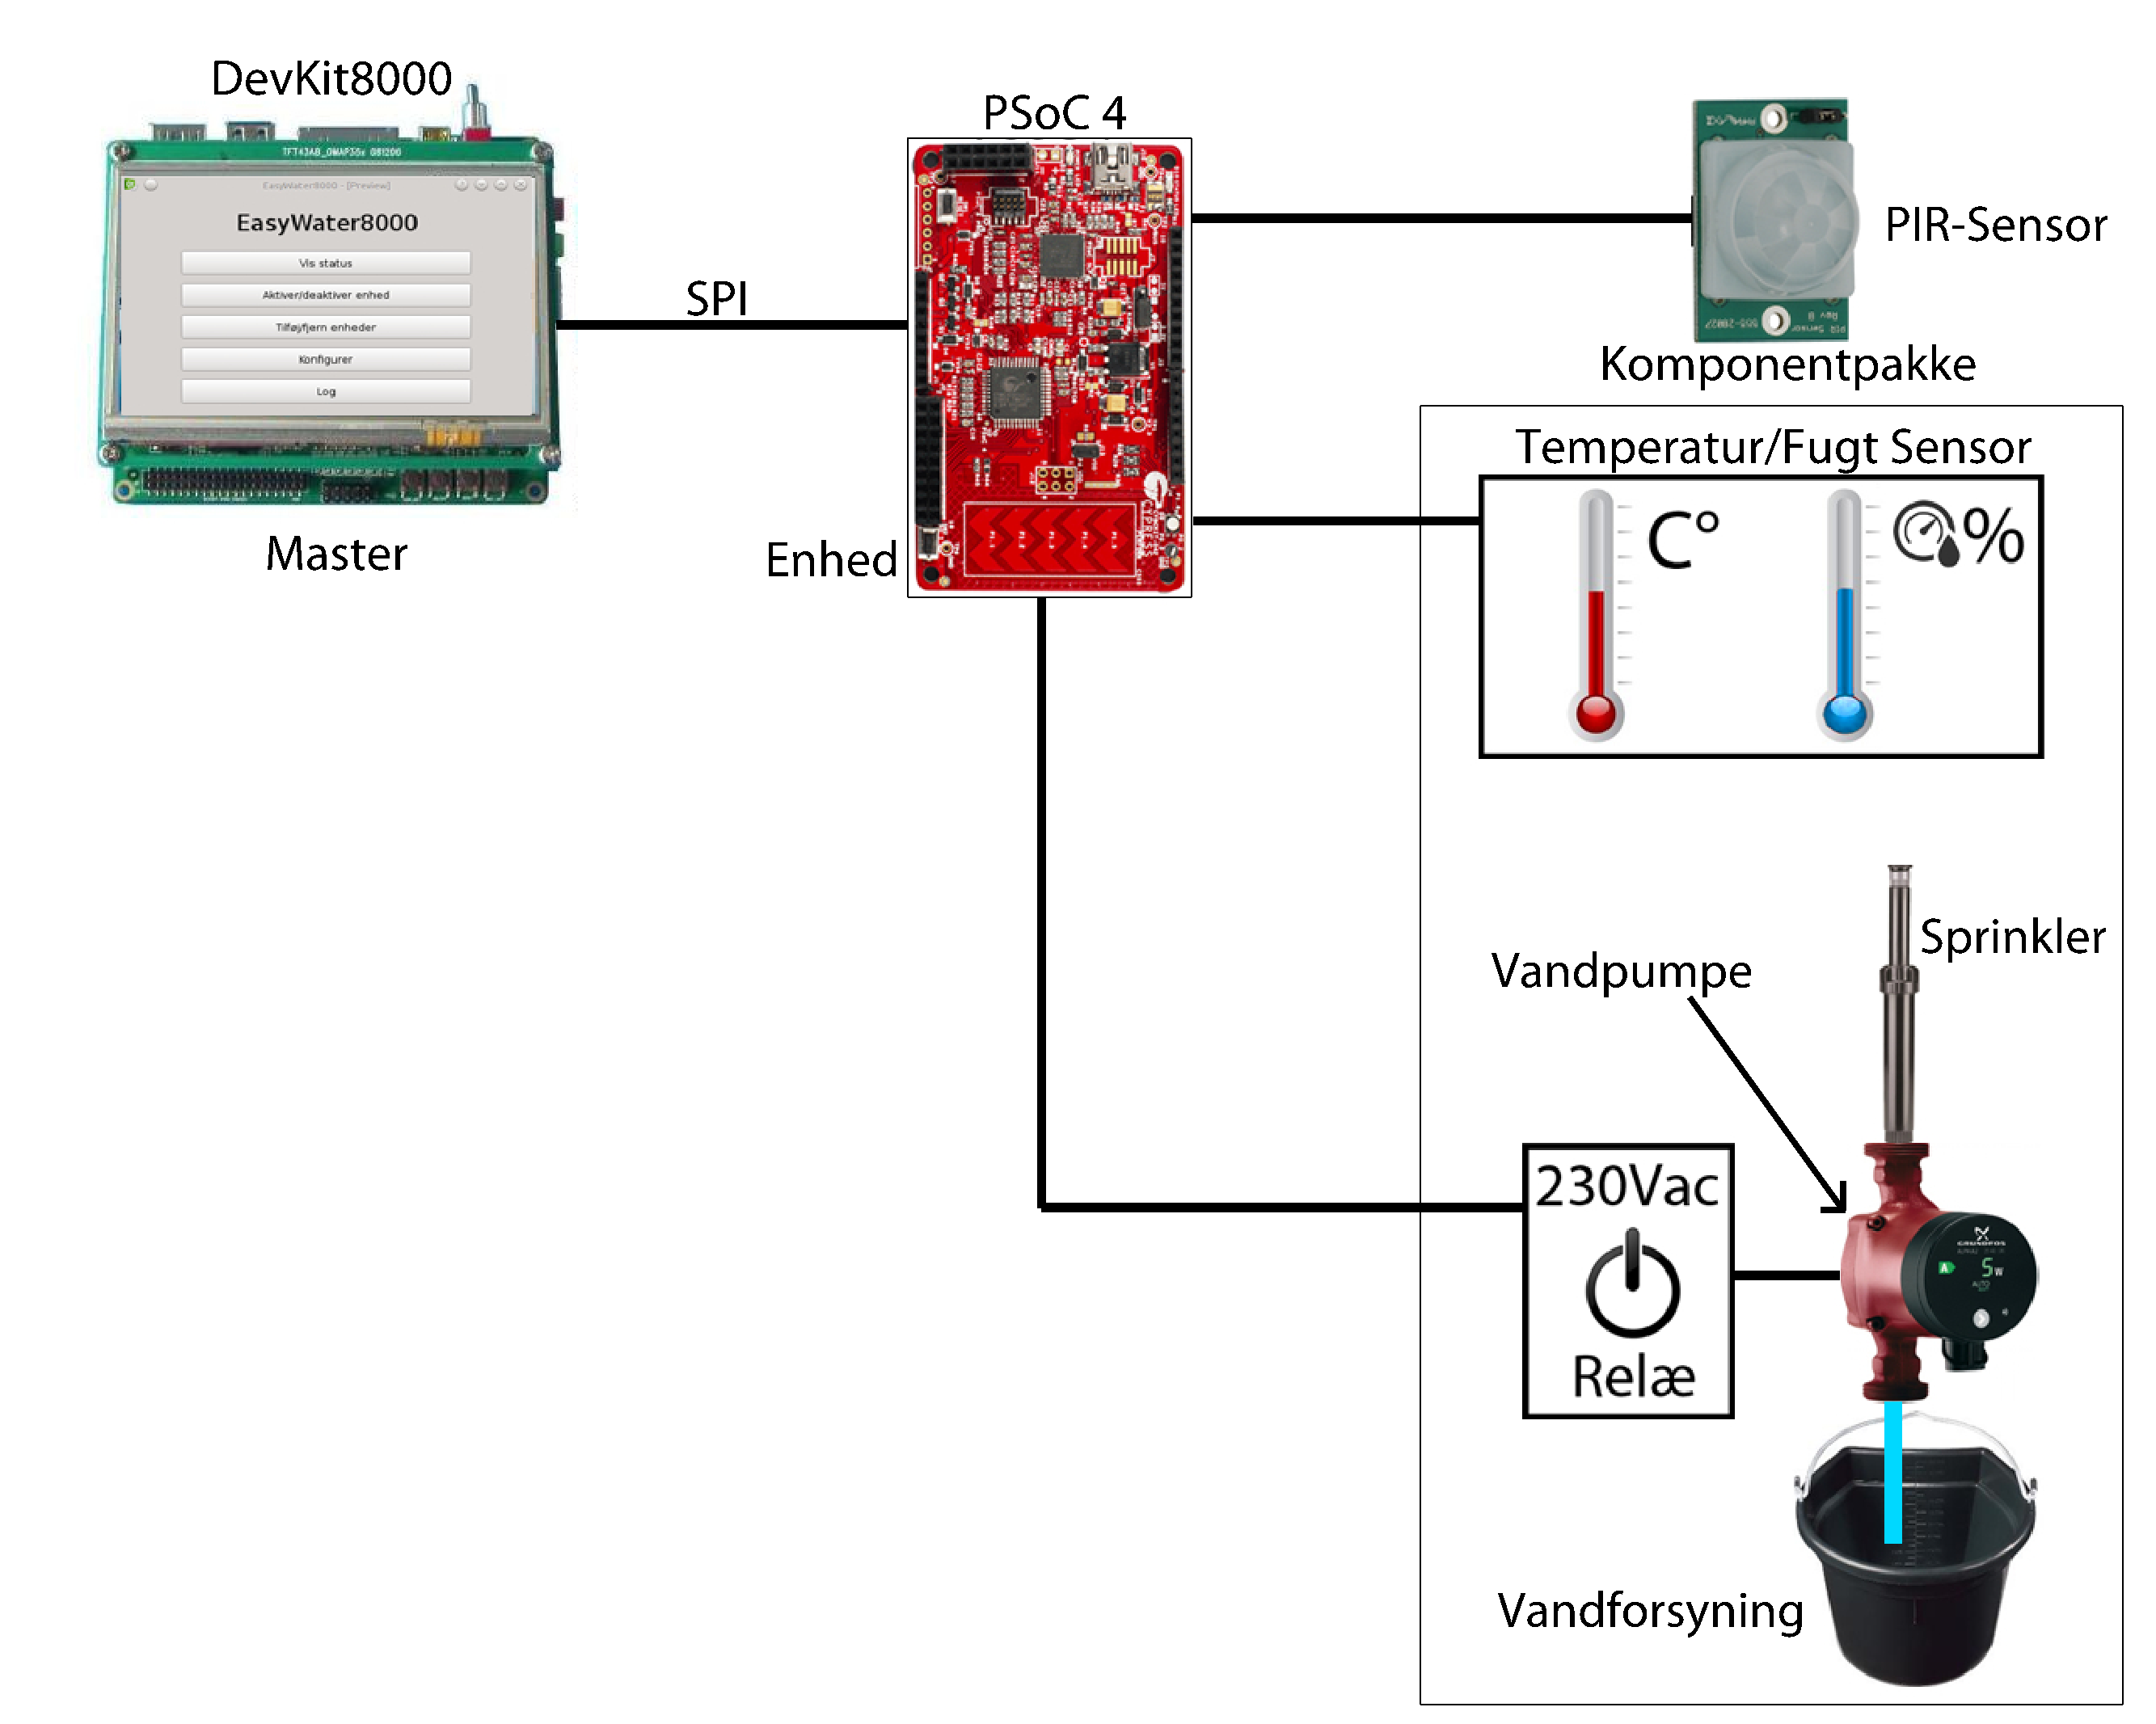
\includegraphics[height=10cm]{filer/indledning/billeder/vandingssystem}} 

Systemet laves med en PSoC som Enhed, altså den del der håndterer data fra sensorene mv.
Devkit8000 fungerer som Masterenhed og er brugerinterface.

En Enhed består altså af:
\begin{enumerate}
\item Fugtighedssensor (evt. flere)
\item Temperatursensor (evt. flere)
\item Bevægelsessensor (evt. flere)
\item Sprinkler (evt. flere)
\item PSoC controller board

\end{enumerate}

Bemærk at der er muligt at forbinde flere af hver type sensore til én enhed. Hvis altså et hul på en golfbane kræver 3 temperatursensorer, kobles disse blot på den samme enhed.

Fugt- og temperatursensorerne registrere banens behov for vanding. Bevægelsessensoren registrere om der er spillerere i umiddelbar nærhed af enheden. Sprinkleren sørger for vandingen. Denne udarbejdes som en motoriseret sprinkler, hvorfra det er muligt at styre i hvilken retning den vander.
PSoC controller boardet bliver hjernen i Enheden. Denne styrer kommunikationen til Masterenheden og holder styr på de generelle funktioner for Enheden så som udlæsning af data, aktivering af sprinkler mv.


{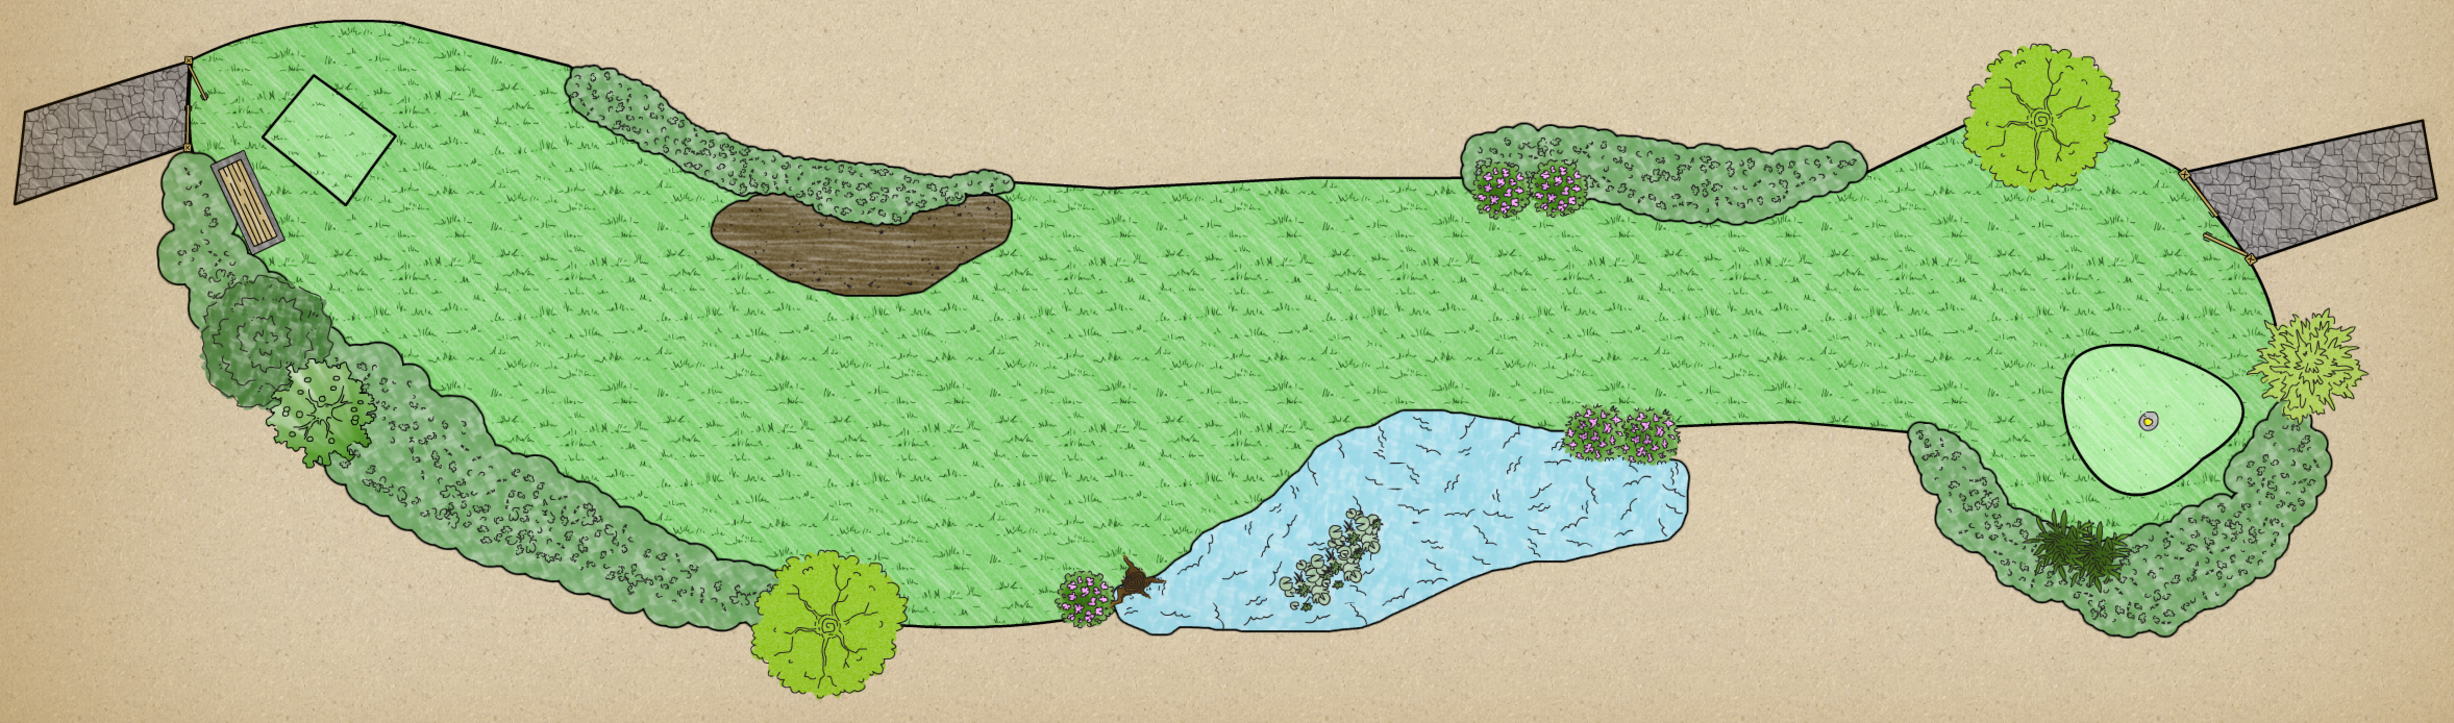
\includegraphics[height=4.2cm]{filer/indledning/billeder/hul_uden_sprinkler}}

{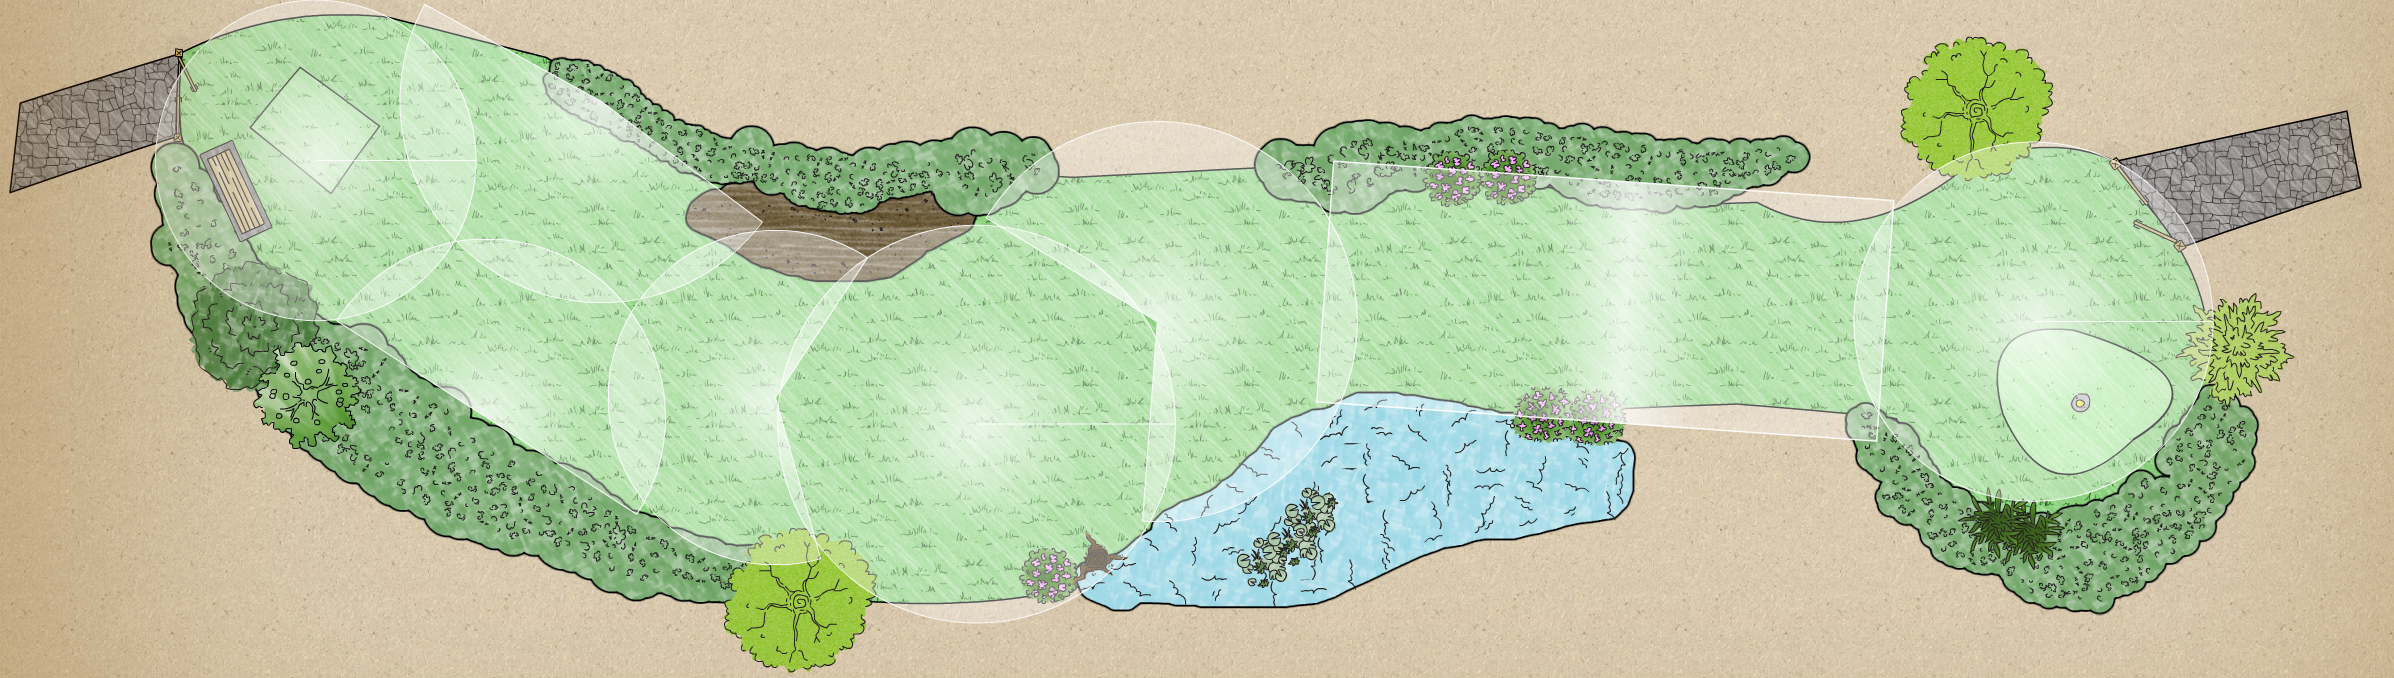
\includegraphics[height=4.1cm]{filer/indledning/billeder/hul_med_sprinkler}}